%%%%%%%%%%%%%%%%%%%%%%%%%%%%%%%%%%%%%%%%%
% Short Sectioned Assignment
% LaTeX Template
% Version 1.0 (5/5/12)
%
% This template has been downloaded from:
% http://www.LaTeXTemplates.com
%
% Original author:
% Frits Wenneker (http://www.howtotex.com)
%
% License:
% CC BY-NC-SA 3.0 (http://creativecommons.org/licenses/by-nc-sa/3.0/)
%
%%%%%%%%%%%%%%%%%%%%%%%%%%%%%%%%%%%%%%%%%

%----------------------------------------------------------------------------------------
%	PACKAGES AND OTHER DOCUMENT CONFIGURATIONS
%----------------------------------------------------------------------------------------

\documentclass[paper=a4, fontsize=11pt]{scrartcl} % A4 paper and 11pt font size

\usepackage[T1]{fontenc} % Use 8-bit encoding that has 256 glyphs
\usepackage{fourier} % Use the Adobe Utopia font for the document - comment this line to return to the LaTeX default
\usepackage[english]{babel} % English language/hyphenation
\usepackage{amsmath,amsfonts,amsthm} % Math packages

\usepackage{lipsum} % Used for inserting dummy 'Lorem ipsum' text into the template

\usepackage{graphicx}

\usepackage{sectsty} % Allows customizing section commands
\allsectionsfont{\centering \normalfont\scshape} % Make all sections centered, the default font and small caps

\usepackage{fancyhdr} % Custom headers and footers
\pagestyle{fancyplain} % Makes all pages in the document conform to the custom headers and footers
\fancyhead{} % No page header - if you want one, create it in the same way as the footers below
\fancyfoot[L]{} % Empty left footer
\fancyfoot[C]{} % Empty center footer
\fancyfoot[R]{\thepage} % Page numbering for right footer
\renewcommand{\headrulewidth}{0pt} % Remove header underlines
\renewcommand{\footrulewidth}{0pt} % Remove footer underlines
\setlength{\headheight}{13.6pt} % Customize the height of the header

\numberwithin{equation}{section} % Number equations within sections (i.e. 1.1, 1.2, 2.1, 2.2 instead of 1, 2, 3, 4)
\numberwithin{figure}{section} % Number figures within sections (i.e. 1.1, 1.2, 2.1, 2.2 instead of 1, 2, 3, 4)
\numberwithin{table}{section} % Number tables within sections (i.e. 1.1, 1.2, 2.1, 2.2 instead of 1, 2, 3, 4)

\setlength\parindent{0pt} % Removes all indentation from paragraphs - comment this line for an assignment with lots of text

%----------------------------------------------------------------------------------------
%	TITLE SECTION
%----------------------------------------------------------------------------------------

\newcommand{\horrule}[1]{\rule{\linewidth}{#1}} % Create horizontal rule command with 1 argument of height

\title{	
\normalfont \normalsize 
\textsc{National Sun Yat-sen University, Department of Mathematics} \\ [25pt] % Your university, school and/or department name(s)
\horrule{0.5pt} \\[0.4cm] % Thin top horizontal rule
\huge Reliability Analysis Assignment 1\\ % The assignment title
\horrule{2pt} \\[0.5cm] % Thick bottom horizontal rule
}

\author{Chia-Hsuan Chang \ and \ Kuan-I Chung} % Your name

\date{\normalsize 2017.03.09} % Today's date or a custom date

\begin{document}

\maketitle % Print the title

%----------------------------------------------------------------------------------------
%	PROBLEM 1
%----------------------------------------------------------------------------------------

\large{Reading Report ------ Reliability in the 21st century (S. Wilson, 2009)}\\

\qquad The reliability analysis can be used widely in many fields including biology, technology and even finance. In biology, this method is applied on survival analysis for estimating hazard ratios and other relevant statistical inferences. It helps insurance companies building up a standard criteria for approving a life insurance and pricing fees. In technology, Reliability is not only used for predicting the life of a chip but also newly utilized in the IT industry for network (including software, hardware and human) degrading detection. In finance, of course, banks and other financial institutions heavily use the reliability for calculating the potential risks caused by financial products.\\

\qquad The reliability is originally applied in the traditional industries for estimating the life of products under the different conditions. For some computational difficulties, the independence assumption is claimed. That is, the
predictors are independent and the models contain no interactions. Yet, practically, the most of the predictors are not independent. For example, in hydrology, considering how storms cause floods, the storms occur under appropriate temperature and humidity such that this three predictors do not meet the assumption of independence. \\

\qquad Besides the contents in the article, we found an example on the internet. Nikon, a world-famous optical product manufacture, launched D700, a full-frame DSLR, in 2008. They claimed that the shutter set tolerates over 150 thousand shots. Thus, Oleg Kikin (https://www.olegkikin.com), a photographer and a blogger built up a website for D700 users such that they could log in two informations, shutter clicks and being dead or not. And the following figure shows the result of Kaplan-Meier survival estimate. \\

\begin{figure}[h] %  figure placement: here, top, bottom, or page
   \centering
   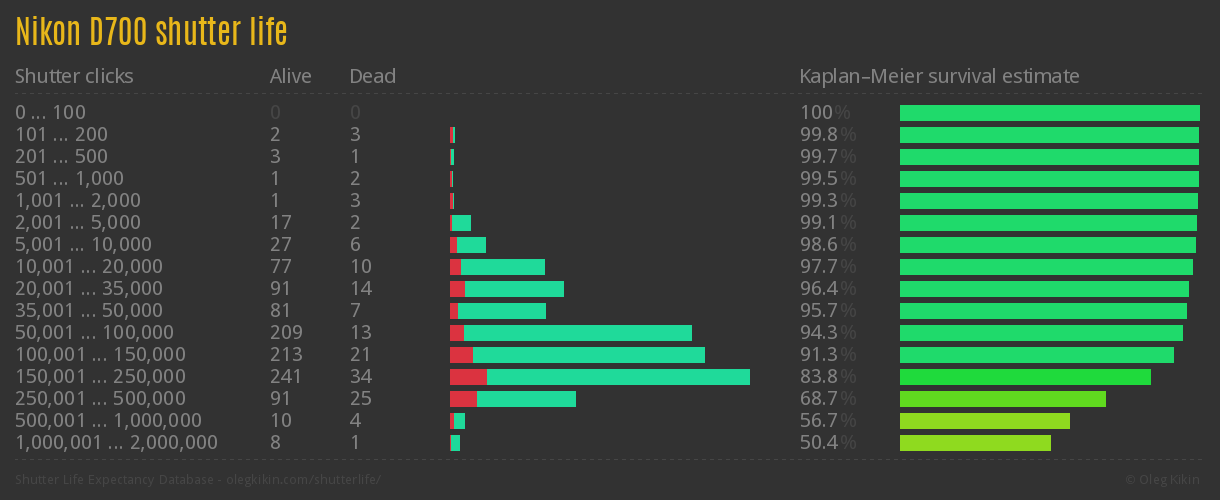
\includegraphics[width=5.78in]{D700.png} 
   \lable{from: https://olegkikin.com/shutterlife/nikon\_d700.htm}
\end{figure}

\qquad We can notice that the K-M method estimates only 91.3\% of shutters sets still function over 150 thousand clicks no matter what the user habits are. Yet, the original factory tested their products by continuous shooting in a severe environment. Thus, this sample survey did not really match what the Nikon claimed. However, the website only considered two variables, the users' habits and the machines' operating environments are excluded. Furthermore, the collected data from the visitors of the website might be impropriate for repeated logging in or maliciously forged logging in which strongly affect the result of the analysis. Hence, the research done by Oleg Kikin might be naive. \\

\qquad Here we want to introduce a concept which could be applied with reliability analysis ------ the music industry. As the internet spreads world-widely, the steaming music services gradually replace the traditional records. Spotify, Apple Music and KK Box record the clicking frequencies of songs. Usually, the clicking frequencies decrease after publishing. Thus, we can analyze the "life time" of songs, discovering the relationship between the clicking rates and the other relevant variables, and then increase the out put value of the entertainment industry.


\end{document}